\chapter{内积空间}
\begin{center}
	% \textcolor[RGB]{255, 0, 0}{\faHeart}所以生命啊,它苦涩如歌.\textcolor[RGB]{255, 0, 0}{\faHeart}
	「花有重开日,人无再少年」
\end{center}
\rightline{——《续侄溥赏酴醾劝酒二首·其一》}
\vspace{-5pt}
\begin{center}
	\pgfornament[width=0.36\linewidth,color=lsp]{88}
\end{center}

\section{内积}

\subsection{向量的点积与长度表示}

本章请读者自行考虑是否阅读,如果读者对线性代数要求不是那么高,可以跳过该章节,本章较有难度,但是看下去会很有意思。

在高中的学习生涯中,我们总是把二维空间$\mathbb{R}^2$与三维空间$\mathbb{R}^3$中的向量具体化为一个有向箭头。通常我们求两点之间的坐标距离会使用勾股定理,在前面的学习中,定义\ref{def:lengthOfVec}就是使用此方法计算的向量长度。

根据定义\ref{def:lengthOfVec}我们可以得到平面上向量$x=(x_1,x_2)$的长度$\left \| x \right \|=\sqrt{x_1^2+x_2^2} $,将等式两边同时平方我们可得$$\left \| x \right \| ^2=x_1^2+x_2^2,$$同时下面定义向量的点积$x \cdot y$:

\begin{definition}{向量的点积(dot product)}
	设$x,y \in \mathbb{R}^n,x=(x_1,x_2,x_3,\cdots,x_n),y=(y_1,y_2,y_3,\cdots,y_n)$则向量$x$与$y$的点积$x\cdot y$定义为$$x\cdot y := x_1y_1+x_2y_2+\cdots+x_ny_n$$
\end{definition}

由于这个概念由实空间出发,所以满足如下公设。

\begin{postulate}
	只有$\mathbb{R}^n$上的向量才能进行点积运算。
\end{postulate}

需要注意的是,点积是将两个向量$x,y\in \mathbb{R}^n$映射为一个实数,所以它们具有如下的性质。

\begin{corollary}
	对于所有的$x,y,z\in \mathbb{R}^n$有:
	\begin{enumerate}
		\item $x\cdot y=y\cdot x$
		\item $x\cdot (y\cdot z)=(x\cdot y)\cdot z$
		\item $x\cdot (y+ z)=x\cdot y+x\cdot z$
		\item 若$T(x,y)=x\cdot y$则$T\in \mathcal{L}((\mathbb{R}^n,\mathbb{R}^n),\mathbb{R})$(表示内积法则操作是线性映射)
		\item $\left \| x \right \| ^2=x\cdot x$
	\end{enumerate}
\end{corollary}

下面的例题可以用于验证上述推论的其中几个。

\begin{example}
	已知点$A(1,3),B(4,1)$在平面直角坐标系中,若向量$x,y,z \in \mathbb{R}^2$,其中$x=\overrightarrow{OA},y=\overrightarrow{OB},z=\overrightarrow{AB}$;
	\begin{enumerate}
		\item 求向量$z$的表示;
		\item 求$\left \| z \right \| ^2$;
		\item 使用勾股定理求线段$AB\footnote{如果没有加任何标记,则表示线段}$的长度
	\end{enumerate}
	\tcblower
	\textcolor{purple}{\textbf{解}}:\begin{enumerate}
		\item $z=y-x,z=(4,1)-(1,3)=(3,-2)$
		\item $\left \| z \right \| ^2=z\cdot z=9+4=13$
		\item 略
	\end{enumerate}
\end{example}

\subsection{内积的定义}

我们刚刚了解了点积,并定义了在实空间上的定义,实际上内积就是点积的推广形式,使其在复空间内可用。我们知道对于一个实数$r\in R$,有$$\left | r \right | =\sqrt{r ^2}$$那么对于一个在二维平面$\mathbb{R}^2$和三维空间$\mathbb{R}^3$中的向量求它的长度,例如$x=(r_1,r_2,r_3)$那么有$$\left \| x \right \| =\sqrt{\left | r_1 \right |^2+\left | r_2 \right |^2+\left | r_3 \right |^2 }$$如果继续向更高维度推广,那么对于$r\in \mathbb{R}^n,r=(r_1,r_2,r_3,\cdots,r_n)$就有$$\left \| r \right \|=\sqrt{\left | r_1 \right |^2+\left | r_2 \right |^2+\left | r_3 \right |^2+\cdots+\left | r_n \right |^2 }$$

那如果我们将其推广到复空间,对于$z=a+b\mathrm{i}$,复空间向量的``长度''\footnote{后面我们会给它一个名字就叫做范数}就可以这样表示,若$z\in \mathbb{C}^n,z=(z_1,z_2,z_3,\cdots,z_n)$那么$$\left \| z \right \|=\sqrt{\left | z_1 \right |^2+\left | z_2 \right |^2+\left | z_3 \right |^2+\cdots+\left | z_n \right |^2 }$$

至于$\left| z \right|^2$如何计算,下面给出复数的模的定义:

\begin{definition}{复数的模,共轭复数}
	复数$z$可以表示为$z=a+b\mathrm{i},a,b\in \mathbb{R}$,我们定义$$\left| z \right|^2:=a^2+b^2$$同时$\left| z \right|^2=(a+b\mathrm{i})(a-b\mathrm{i})$,而$a-b\mathrm{i}$我们称其为$z$的共轭复数,记作$\overline{z}$,所以我们有$$\left| z \right|^2=z\overline{z}$$
\end{definition}

所以$z\in \mathbb{C}^n,z=(z_1,z_2,z_3,\cdots,z_n)$,根据到复空间的推广和复数的模的定义可得$$\left \| z \right \| =\sqrt{z_1\overline{z_1}+z_2\overline{z_2}+z_3\overline{z_3}+\cdots+z_n\overline{z_n}}$$

推广到复空间的向量点积我们称其为内积,如果我们将范围限定在$\mathbb{R}^n$上对两个向量进行操作,那么实空间上的内积就是点积,下面我们给出定义:

\begin{definition}{内积的定义}
	若向量$a,b\in \mathbb{C}^n,a=(z_1,z_2,z_3,\cdots,z_n),b=(c_1,c_2,c_3,\cdots,c_n)$那么它们的内积记作$\left \langle a , b \right \rangle $表示为$$\left \langle a , b \right \rangle :=z_1\overline{c_1}+z_2\overline{c_2}+z_3\overline{c_3}+\cdots+z_n\overline{c_n}$$
\end{definition}

我们知道,$c\in \mathbb{R},c=a+0\mathrm{i}$,所以$\left| c \right|^2=c^2$,所以说实空间上面的内积就是点积。

\begin{corollary}
	\label{cor:innerProduct}
	$V$是$\mathbb{C}$上的线性空间,向量$u,v\in V$,标量$\lambda \in \mathbb{C}$对于其内积$\left \langle u,v \right \rangle $有如下性质
	\begin{enumerate}
		\item 正性(positivity):对于所有的$v$,$\left \langle v,v \right \rangle\ge 0 $;
		\item 定性(definiteness):当且仅当$v=0$时$\left \langle v,v \right \rangle= 0 $;
		\item 对第一变量的线性(linearly for first slot):$\lambda \left \langle u,v \right \rangle=\left \langle \lambda u,v \right \rangle,\left \langle u+w,v \right \rangle=\left \langle u,v \right \rangle+\left \langle w,v \right \rangle$;
		\item 共轭对称性(conjugate symmetry):$\left \langle u,v \right \rangle= \overline{\left \langle v,u \right \rangle} $。
	\end{enumerate}
\end{corollary}

\begin{example}
	求证:对所有的$u,v,w \in \mathbb{C}^n$都有$\left \langle u,v+w \right \rangle =\left \langle u,v \right \rangle +\left \langle u,w \right \rangle $
	\tcblower
	\textcolor{purple}{\textbf{解}}:根据共轭对称性,则有$$\left \langle u,v+w \right \rangle =\overline{\left \langle v+w,u \right \rangle } $$根据内积的定义,有$$\overline{\left \langle v+w,u \right \rangle } =\overline{\left \langle v,u \right \rangle } +\overline{\left \langle w,u \right \rangle }$$再根据共轭对称性有$$\overline{\left \langle v,u \right \rangle } +\overline{\left \langle w,u \right \rangle }=\left \langle u,v \right \rangle +\left \langle u,w \right \rangle $$这证明了内积的第二个变量也满足线性。
\end{example}

\subsection{范数}

我们把之前所有实空间长度和复空间$v\in \mathbb{C}^n$与自身的内积$\left \langle v,v \right \rangle $赋予一个新名词叫做范数,它的定义如下:

\begin{definition}{范数(norm)}
	对于$v\in V$那么$v$的范数$\left \| v \right \| $定义为$$\left \| v \right \| :=\sqrt{\left \langle v,v \right \rangle }$$
\end{definition}

\subsection{内积空间}

本章节主要研究内积空间,所以我们做出如下定义:

\begin{definition}{内积空间}
	若线性空间$H$有$x,y,z\in H$使得在$H$上存在函数$f(x,y)=z$,它们满足下面的内积映射条件$$f: (H,H)\rightarrow \mathbb{C}$$其中$$f(x,y)=\left \langle x,y \right \rangle =z$$那么称$H$为内积空间\footnote{完备的内积空间称为Hilbert(希尔伯特)空间}并满足推论\ref{cor:innerProduct}的相关性质。
\end{definition}

\begin{ascolorbox1}{思考}
	内积空间是否是线性空间?
\end{ascolorbox1}

答案是一定是线性空间,留给读者自己思考并查阅相关资料证明。

至于内积空间它能够干什么,下面给出通过内积空间衍生的几个著名不等式。

\subsection{Cauchy-Schwarz 不等式}
%cite
首先我们来看 Cauchy-Schwarz\footnote{一般译作柯西-施瓦茨} 不等式。

\begin{theorem}{Cauchy-Schwarz 不等式}
	设内积空间$H$中有$v,w\in H$则有如下不等式成立:$$\left | \left \langle u,v \right \rangle  \right | \le \left \| u \right \| \left \| v \right \| $$当且仅当$u=\lambda v,\lambda \in \mathbb{F}$。
\end{theorem}

\begin{proof}
	由正性与定性\footnote{可以合起来,叫做正定性}可得,对于任意的$x,y\in H,\lambda \in \mathbb{F}$有$$\left \langle x+\lambda y,x+\lambda y \right \rangle \ge 0$$由共轭对称性可知$$\left \langle x+\lambda y,x+\lambda y \right \rangle=\overline{\left \langle x+\lambda y,x+\lambda y \right \rangle}$$将其展开可得$$\left \langle x+\lambda y,x+\lambda y \right \rangle =\left \langle x,x \right \rangle +\overline{\lambda} \left \langle x,y \right \rangle +\lambda \left \langle y,x \right \rangle+\left | \lambda \right |^2\left \langle y,y \right \rangle \ge 0$$首先考虑$y=0$的情况,$(\left \langle x,0 \right \rangle )^2=0,\left \langle x,x \right \rangle =x,\left \langle 0,0 \right \rangle =0$等号严格成立,若$y\neq 0$令$\displaystyle \lambda =-\frac{\left \langle x,y \right \rangle }{\left \langle y,y \right \rangle }$并带入可以证明。$\square$
\end{proof}

下面是 Cauchy-Schwarz 不等式的两种形式,其中第一种是法国数学家Augustin Louis Cauchy\footnote{一般译作:奥古斯丁$\cdot$路易斯$\cdot$柯西}在1821年证明,第二个由德国数学家Hermann Amandus Schwarz\footnote{一般译作:赫尔曼$\cdot$阿曼杜斯$\cdot$施瓦茨}在1886年证明。

\begin{corollary}
	\begin{enumerate}
		\item 若$x_1,x_2,x_3,\cdots,x_n,y_1,y_2,y_3,\cdots,y_n\in \mathbb{R}$则有$$\left( x_1y_1+x_2y_2+\cdots+x_ny_n \right)^2\le \left( x_1^2+x_2^2+x_3^2+\cdots+x_n^2 \right)\left( y_1^2+y_2^2+y_3^2+\cdots+y_n^2 \right)$$写成求和符号就是$$\left ( \sum_{i=1}^{n}x_iy_i  \right ) ^2\le \left ( \sum_{i=1}^{n}x_i^2  \right ) \left ( \sum_{i=1}^{n}y_i^2  \right ) $$
		\item 设$f,g$在$\left [ -1,1 \right ] $上连续,则$$\left ( \int_{-1}^{1}f(x)g(x)\mathrm{d}x \right )  ^2\le \left ( \int_{-1}^{1}\left ( f(x) \right )^2 \mathrm{d}x \right ) \left ( \int_{-1}^{1}\left ( g(x) \right )^2 \mathrm{d}x \right ) $$
	\end{enumerate}
\end{corollary}

\subsection{余弦定理}

在二维空间$\mathbb{R}^2$和三维空间$\mathbb{R}^3$的空间中,有一条余弦定理,它能够帮助我们解三角形,定理如下。
%cite
\begin{theorem}{余弦定理}
	在三角形内,设$a,b$为角$C$的邻边,$c$为角$C$的对边,则它们满足$$c^2=a^2+b^2-2ab\cos C$$
\end{theorem}

读者可使用几何法尝试验证,留作练习。

下面我们对其进行推广,我们可以得到内积空间上的余弦定理,同时有内积公式。

\begin{corollary}
	若$a,b \in H$则有$$\left \| c \right \| ^2=\left \| a \right \| ^2+\left \| b \right \| ^2-2\left \langle a,b \right \rangle $$
\end{corollary}

为了更好的引入内积公式,下面我们定义$\mathbb{C}^n$上的两向量的夹角的值。

\begin{definition}{两向量夹角的值}
	若$a,b\in \mathbb{C}^n$则$a,b$的夹角$\varphi$满足$$\varphi := \cos^{-1}\frac{\left \langle a,b \right \rangle }{\left \| a \right \| \left \| b \right \| }$$
\end{definition}

请读者举例验证在$\mathbb{R}^2,\mathbb{R}^3$上的正确性,并使用余弦定理证明在$\mathbb{R}^2,\mathbb{R}^3$的正确性。

\begin{example}
	给出复变反余弦函数的公式:若$z\in \mathbb{c}$那么其反余弦的值为$$\cos^{-1} z=-\mathrm{i}+\ln \left( z+ \mathrm{i} \sqrt{1-z^2}\right)$$
	利用上述公式计算:已知$a,b \in \mathbb{C}^n,a=(\mathrm{i},2\mathrm{i},3),b=(1,2,3\mathrm{i})$求向量$a,b$的夹角的余弦值$\varphi$。
	\tcblower
	\textcolor{purple}{\textbf{解}}:根据定义,计算$\left \langle a,b \right \rangle =\mathrm{i}+4\mathrm{i}-9\mathrm{i}=-4\mathrm{i} ,\left \| a \right \| =\left \| b \right \|=\sqrt{14}$所以$$\varphi =\cos ^{-1} \left( -\frac{2}{7}\mathrm{i} \right)$$带入上述公式,可得$$\varphi=-\mathrm{i}+\ln \left( -\frac{2}{7}\mathrm{i}+\mathrm{i}\sqrt{1+\frac{4}{49}} \right)$$实数部分化简后可得$$\varphi=-\mathrm{i}+\ln \left( \frac{\sqrt{53}-2}{7}\mathrm{i} \right)\footnote{由于这本书不讲复变,所以就化简至此,不取其主值。}$$
\end{example}

下面给出内积公式。

\begin{theorem}{内积公式}
	若$u,v \in \mathbb{C}^n$,$\varphi$为$u,v$的夹角,那么它们的内积表示为$$\left \langle u,v \right \rangle =\left \| u \right \| \left \| v \right \| \cos \varphi$$
\end{theorem}

根据两向量夹角的值代入可以轻松证明该定理成立,或使用余弦定理证明在$\mathbb{R}^2,\mathbb{R}^3$上的正确性。

\subsection{三角不等式}
%pic
如图\ref{fig:TrangleIneq},我们都知道,三角形两边之和大于第三边,在二维空间$\mathbb{R}^2$和三维空间$\mathbb{R}^3$的空间中\footnote{这里的空间体系都是欧几里得体系},这是作为一条公理存在的,即:

\begin{figure}[htbp]
	\centering
	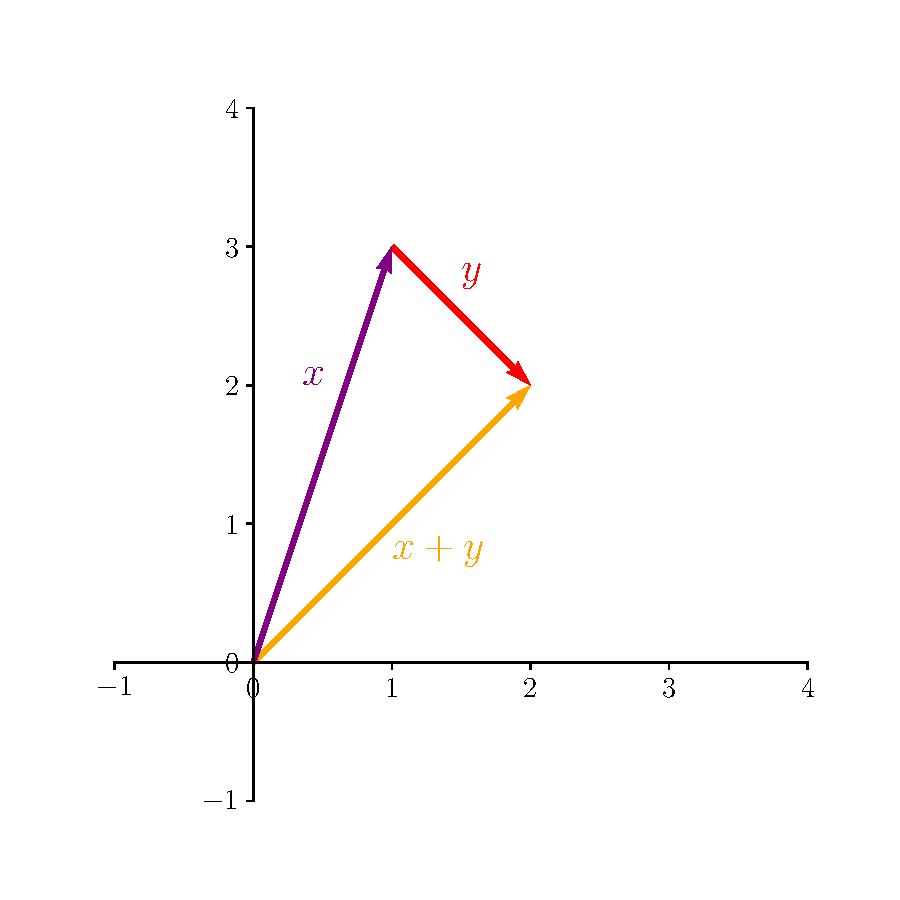
\includegraphics[width=0.4\linewidth]{figure/eps/TrangleIneq.eps}
	\caption{三角不等式}
	\label{fig:TrangleIneq}
\end{figure}

\begin{axiom}{平面长度最短公理}
	在平面内,两点之间,线段最短。
\end{axiom}

如果将其推广到内积空间,则有如下不等式成立:

\begin{theorem}{三角不等式}
	若$u,v\in H$,则$$\left \| u+v \right \| \le \left \| u \right \| +\left \| v \right \| $$当且仅当$u=\lambda v,\lambda>0$等号成立。
\end{theorem}

\begin{proof}
	首先根据范数的定义,我们可以得到$$\left \| u+v \right \|^2 =\left \langle u+v,u+v \right \rangle $$根据两个变量的线性,我们可以得到$$\left \langle u+v,u+v \right \rangle =\left \langle u,u \right \rangle +\left \langle v,v \right \rangle +\left \langle u,v \right \rangle +\left \langle v,u \right \rangle $$根据共轭对称性可得$$\left \langle u+v,u+v \right \rangle =\left \langle u,u \right \rangle +\left \langle v,v \right \rangle +\left \langle u,v \right \rangle +\overline{\left \langle u,v \right \rangle} $$化简并合并可得$$\left \| u+v \right \|^2=\left \| u \right \| ^2+\left \| v \right \| ^2+2\text{Re}\left \langle u,v \right \rangle \footnote{若$x=a+b\mathrm{i}$那么$\text{Re}(x)$表示取$x$的实数部分$a$,$\text{Im}(x)$表示取$x$的虚数部分$b$}$$适当取放缩可得$$\left \| u+v \right \|^2\le \left \| u \right \| ^2+\left \| v \right \| ^2+2\left | \left \langle u,v \right \rangle  \right | $$根据Cauchy-Schwarz不等式可得$$\left \| u \right \| ^2+\left \| v \right \| ^2+2\left | \left \langle u,v \right \rangle  \right | \le \left \| u \right \| ^2+\left \| v \right \| ^2+2\left \| u \right \|\left \| v \right \|$$最后我们合并不等式右侧,可得$$\left \| u+v \right \|^2 \le \left( \left \| u \right \| +\left \| v \right \|  \right)^2$$
	两边开二次根即可得证。$\square$
\end{proof}

\section{正交}

\subsection{正交的定义}

根据内积公式$\left \langle u,v \right \rangle =\left \| u \right \| \left \| v \right \| \cos \varphi$,特别地,两个向量的内积等于0的时候我们有一个关键的定义:正交。

\begin{definition}{正交(orthogonal)的定义}
	若向量$a,b \in H$有$\left \langle a,b \right \rangle = 0$则称$a,b$是正交的\footnote{有些教材会使用$a,b$是垂直的}。
\end{definition}

通常来讲,向量的范数不为0,当$\cos \varphi$为0的时候两个向量正交;也就是说,通常两个向量的夹角为$\displaystyle \frac{\pi}{2}$的时候两个向量正交。

对于向量$\boldsymbol{0}$我们有如下推论:

\begin{corollary}
	\begin{enumerate}
		\item $\boldsymbol{0}$与$H$中的任何向量正交;
		\item $\boldsymbol{0}$与自身正交。
	\end{enumerate}
\end{corollary}

\subsection{正交基}

首先是正交基的概念,若基集合$\left\{ a_1,a_2,a_3\cdots,a_n \right\}$是正交基,则该基的元素两两正交。

\begin{definition}{正交基(orthonormal basis)}
	若内积空间$H$上的基$S=\left\{ a_1,a_2,a_3\cdots,a_n \right\}$满足对于任意一个$i,j \in \mathbb{N}^+$且$i\neq j$使得$$\left \langle a_i,a_j \right \rangle =0$$我们称$S$为空间$H$的正交基。
\end{definition}

举个例子,$\mathbb{R}^3$的正交基可以是$\left\{ (0,0,1),(0,1,0),(1,0,0) \right\}$。

\subsection{Gram-Schmidt 正交化}

在前面的学习中,若线性空间$V$的基为$S=\left\{ a_1,a_2,a_3,\cdots,a_n \right\}$那么对于任意一个$v\in V$都可以使用$S$的线性组合表示,即对于任何一个$v \in V$存在$\lambda_1,\lambda_2,\lambda_3,\cdots,\lambda_n$满足下面的式子成立。$$v=\lambda_1a_1+\lambda_2a_2+\lambda_3a_3+\cdots+\lambda_na_n$$由于正交基是一种特殊的基,所以它们也满足该性质,我们有如下的等式来描述它们的线性组合表示的向量,称作正交分解。

\begin{theorem}{正交分解(orthogonal decomposition)}
	\label{the:orthogonalDecomposition}
	设内积空间$V$上的基为$S=\left\{ a_1,a_2,a_3,\cdots,a_n \right\}$,则对于任何一个$v\in V$满足等式$$v=\left \langle v,a_1 \right \rangle a_1+\left \langle v,a_2 \right \rangle a_2+\cdots+\left \langle v,a_n \right \rangle a_n$$成立,写成求和符号就是$$v=\sum_{i=1}^{n} \left \langle v,a_i \right \rangle a_i$$并同时满足$$\left \| v \right \| ^2=\sum_{i=1}^{n}\left( \frac{\left | \left \langle v,a_i \right \rangle  \right |}{\left \| a_i \right \|} \right)^2$$
\end{theorem}

我们还是从$\mathbb{R}^2$和$\mathbb{R}^3$入手考虑,通常在我们高中的物理学习中会学到力的分解,下面是在$\mathbb{R}^2$上的图形直观的解释。

\begin{figure}[htbp]
	\centering
	
\begin{tikzpicture}[yscale=1,xscale=1,line width=0.8pt]
    \draw (0,0) rectangle (4,2);
    \draw[->,>=Stealth] (2,1)--(6,3)node[above=2.5pt,right=2.5pt]{$F$};

	\draw[->,>=Stealth,dashed] (2,1)--(2,3)node[above=2.5pt,right=2.5pt]{$F_{\text{垂直}}$};

    \draw[->,>=Stealth,dashed] (2,1)--(6,1)node[above=2.5pt,right=2.5pt]{$F_{\text{平行}}$};

    \coordinate (O) at (2,1);
    \coordinate (A) at (3,1.5);
    \coordinate (B) at (3,1);
    \draw pic["$\varphi$",draw,angle radius=1cm,angle eccentricity=1.4] {angle = B--O--A};
\end{tikzpicture}
	\caption{力的合成与分解}
	\label{tikz:force}
\end{figure}

如图\ref{tikz:force}所示,$F_{\text{垂直}}$和$F_{\text{平行}}$是正交的,我们可以将$F$分解为这两个向量,根据内积公式,$\left \langle F,F_{\text{平行}} \right \rangle =\left \| F \right \| \left \| F_{\text{平行}} \right \|\cos \varphi $所以分解为$F_{\text{平行}}$的分量可以使用正交分解公式,同理$F_{\text{垂直}}$也是如此,这样一来可以将$F$分解为两个正交基的和即$$F=F_{\text{垂直}}+F_{\text{平行}}$$

同理,在$\mathbb{R}^n$上的向量均可使用定理\ref{the:orthogonalDecomposition}使其正交化;而下面要讲的一个内容表示的是,可以将一些线性无关的向量正交化,使其两两正交。且正交化后张成的空间与原向量张成的空间相同,这就是 Gram-Schmidt\footnote{一般译作格拉姆-施密特,由两位数学家的名字构成,分别是丹麦数学家Jørgen Pedersen Gram和德国数学家Erhard Schmidt} 正交化过程。
%cite

\begin{theorem}{Gram-Schmidt 正交化}
	设向量$S=\left\{ v_1,v_2,v_3,\cdots,v_n \right\}$线性无关,存在向量$S'=\left\{ a_1,a_2,a_3,\cdots,a_n \right\}$为正交基,并满足
	$$a_k=v_k-\sum_{i=1}^{k-1} \frac{\left \langle a_i,v_k \right \rangle }{\left \langle a_i,a_i \right \rangle }a_i $$
	成立,且$$\text{Span}(S)=\text{Span}(S')$$
\end{theorem}

下面是一个利用 Gram-Schmidt 正交化的一个例子。

\begin{example}
	在三维空间$\mathbb{R}^3$中,有一组基$\left\{ a_1,a_2,a_3 \right\}$,其中$a_1=(1,1,1),a_2=(1,1,0),a_3=(1,0,0)$请使用 Gram-Schmidt 正交化将其转化为$S'=\left\{ v_1,v_2,v_3 \right\}$,$S'$为$\mathbb{R}^3$的正交基。
	\tcblower
	\textcolor{purple}{\textbf{解}}:根据 Gram-Schmidt 正交化依次可得\begin{align}
		&v_1=a_1=(1,1,1)\\&v_2=a_2-\frac{\left \langle v_1,a_1 \right \rangle }{\left \langle v_1,v_1 \right \rangle }v_1=(0,1,1)-\frac{2}{3}(1,1,1)=\left( -\frac{2}{3},\frac{1}{3},\frac{1}{3} \right)\\&v_3=a_3-\frac{\left \langle v_1,a_3 \right \rangle }{\left \langle v_1,v_1 \right \rangle }v_1-\frac{\left \langle v_2,a_3 \right \rangle }{\left \langle v_2,v_2 \right \rangle }v_2\notag\\&v_3=(0,0,1)-\frac{1}{3}(1,1,1)-\frac{1/3}{2/3}\left( -\frac{2}{3},\frac{1}{3},\frac{1}{3}  \right)=\left( 0,-\frac{1}{2},\frac{1}{2} \right)
	\end{align}
\end{example}

\begin{ascolorbox1}{思考}
	如果向量$S$线性相关,如果对其使用 Gram-Schmidt 正交化会发生什么?
\end{ascolorbox1}

答案是最后一个向量正交化后会变为$\boldsymbol{0}$向量,它们确实两两正交,不过$\boldsymbol{0}$向量不能成为基的一个。

读者不难发现,向量在正交化的时候也相当于一个线性映射,即原向量$v_i$被映射为了$a_i$,同时也不难发现这是一个从自己空间映射到自己空间的映射,我们给它一个名称叫做算子(operator)。

\begin{definition}{算子(operator)}
	线性映射从$V$到$V$的集合$\mathcal{L}(V,V)$中的元素称作$V$上的算子,我们把线性映射到本身的集合简写为$\mathcal{L}(V)$。
\end{definition}

例如线性映射,$T((x,y))=(y,x)$,$T$就是$\mathbb{R}^2$上的算子,因为映射前后的空间都是$\mathbb{R}^2$,可以写作$T\in \mathcal{L}(\mathbb{R}^2)$。

回到刚刚所说的原向量$v_i$被映射为了$a_i$,若映射法则$T$将$v_i$被映射为了$a_i$,如果我们将此线性映射表示为矩阵积,那么它应当满足:$$\begin{pmatrix}
	a_1& a_2 & a_3 & \cdots & a_n
  \end{pmatrix}=\begin{pmatrix}
	v_1& v_2 & v_3 & \cdots & v_n
\end{pmatrix}\mathcal{M}(T)\footnote{这种写法用向量的矩阵表示,即若$a_i,v_i\in \mathbb{R}^m$则这两个是$m\times n$的矩阵}$$在正交化这样的过程中,我们可以得到$\mathcal{M}(T)$是上三角矩阵,即$$\begin{pmatrix}
	a_1& a_2 & a_3 & \cdots & a_n
  \end{pmatrix}=\begin{pmatrix}
	v_1& v_2 & v_3 & \cdots & v_n
	\end{pmatrix}=\begin{pmatrix}  
	1 & * & \cdots &* & * \\  
	0 & * & \cdots &* & * \\  
	\vdots & \vdots & \ddots & \vdots & \vdots \\  
	0 & 0 & \cdots & 0 & * 
  \end{pmatrix} $$

\subsection{正交投影}

想象一下在$\mathbb{R}^3$中,有一条直线和一个平面垂直,在高中的学习生涯中我们知道在平面上任意取一个有向箭头,都与这条直线垂直,换句话说,平面上所有有向箭头表示的向量都与这条直线的方向向量正交。

所以我们引入一个正交补空间,表示该空间内向量对一个子空间中的任意一个向量正交,下面我们给出定义:

\begin{definition}{正交补空间}
	设子空间$U$中的向量均与子空间$V$中的向量正交,我们称$V$是$U$的正交补空间,并有一个符号$U^{\bot}$表示;即$$U^{\bot}:=\left\{ a\in V\mid \forall\footnote{符号$\forall$ 表示对于所有的,这个集合的描述为,$U^{\bot}$集合的元素$a\in V$对于所有的$u \in U$的使得$\left \langle u,a \right \rangle =0$成立} u\in U\Longrightarrow \left \langle u,a \right \rangle =0 \right\}$$
\end{definition}

\begin{figure}[htbp]
	\centering
	\tdplotsetmaincoords{70}{100}

\begin{tikzpicture}[yscale=1,xscale=1,line width=0.8pt,tdplot_main_coords]
	\coordinate (A) at (0,0,0);
	\coordinate (B) at (4,0,0);
    \coordinate (C) at (4,4,-2);
    \coordinate (D) at (0,4,-2);

    \coordinate (L1) at (2,3,1);
    \coordinate (L2) at (2,1,-3);

    \draw (L1)--(L2) node[above=3.5pt,right=3pt]{$l$};
    
    \fill[pink!40!white,opacity=0.6] (A)--(B)--(C)--(D)--cycle;
    \draw (B)node[above=3.5pt,right=3pt]{$\alpha$};
	%\draw(P)node[above=3.5pt,right=3pt]{$P$};
\end{tikzpicture}
	\caption{正交补空间}
	\label{tikz:botspace}
\end{figure}

如图\ref{tikz:botspace}所示,$\mathbb{R}^3$上满足$l \bot \alpha$所以$l$和$\alpha$表示的线性空间相互正交补,即$\alpha^{\bot}=l,l^{\bot}=\alpha$,由此我们引入正交投影的概念,并解决一些极小化问题。

\begin{definition}{正交投影(orthogonal projection)}
	设$V$的一个有限维子空间为$U$,定义$V$到$U$上的正交投影为$P_{U}\in \mathcal{L}(V)$为对所有的$v\in V$均可写成$v=u+w$,其中$u\in U$且$w\in U^{\bot}$,则$P_U(v)=w$,向量$w$称为$v$在$U$上的投影。
\end{definition}

结合我们之前讲过的线性映射的零空间和值域空间,便有如下推论。

\begin{corollary}
	若$U$是$V$的有限维子空间,则$P_U\in \mathcal{L}(V)$满足$$\text{range}P_U=\left( \text{null} P_U \right)^{\bot}=U$$
\end{corollary}

\section{极小化问题}

\subsection{到子空间的最短距离}

还是在高中的学习生涯中我们遇到过在空间$\mathbb{R}^3$上给定一个点,并求它到直线或平面的最短距离,为了后续抽象化的操作,我们先来定义什么是点。

\begin{definition}{点(point)与点的距离(point distance)}
	子空间$V$上的点$v\in V$是一个向量,在图形中通常表示为从 $\boldsymbol{0}$开始的有向箭头。若两个不相同的点$v,w \in V$则它们的距离表示为$$d(v,w) := \left \| v-w \right \| \footnote{在这一部分,我们都用欧几里得体系表示空间}$$
\end{definition}

例如在$\mathbb{R}^2$中点$v=(3,4)$和点$w=(0,1)$的距离为$d(v,w)=\sqrt{3^2+3^2}=3\sqrt{2}$,根据定义我们可以把上面的问题描述成:给定一个空间$V$的子空间$U$和点$v\in V$,求点$u\in U$使得$\left \| v-u \right \| $最小;在解决该问题的策略中,我们知道点到直线或平面的距离最短的情况应该是垂直到点的情形,所以到子空间的最小距离应当是到该子空间正交补空间上取点,下面的一个命题表示将点通过$P_U$映射到子空间后点的距离最短。

\begin{theorem}{到子空间的最短距离}
	设$U$为$V$有限维子空间,有$v\in V$且$u\in U$那么$$\left \| v-P_U(v) \right \| \le \left \| v-u \right \| $$
\end{theorem}

\begin{figure}[htbp]
	\centering
	\begin{tikzpicture}[yscale=1,xscale=1,line width=0.8pt]
	\coordinate (A) at (-1,-1);
	\coordinate (B) at (4,4);
    \coordinate (O) at (0,0);
    \coordinate (V) at (1,3);
    \coordinate (P) at (2,2);
    \draw (A)--(B) node[above=3.5pt,right=3pt]{$U$};
    \draw[->,>=Stealth](O)--(V)node[above=2.5pt,left=1.5pt]{$v$};
    \draw[->,>=Stealth](O)--(P)node[above=2.5pt,right=1.5pt]{$P_U(v)$};
    \filldraw[black] (O) circle (2pt) node[anchor=west]{$O$};
    \draw (P)--(V);
	%\draw(P)node[above=3.5pt,right=3pt]{$P$};
\end{tikzpicture}
	\caption{$P_U(v)$是$v$的最短距离}
	\label{tikz:botDistanceLine}
\end{figure}

\subsection{多项式与极小化}

